\documentclass{beamer}
\usepackage[utf8]{inputenc}

\usetheme{Boadilla}
\usecolortheme{lily}
\usepackage{amsmath,amssymb,amsfonts,amsthm}
\usepackage{mathtools}
\usepackage{txfonts}
\usepackage{tkz-euclide}
\usepackage{listings}
\usepackage{multicol}
\usepackage{adjustbox}
\usepackage{array}
\usepackage{tabularx}
\usepackage{lmodern}
\usepackage{gvv}
\usepackage{circuitikz}
\usepackage{tikz}
\usepackage{graphicx}

\setbeamertemplate{footline}
{
  \leavevmode%
  \hbox{%
  \begin{beamercolorbox}[wd=\paperwidth,ht=2.25ex,dp=1ex,right]{author in head/foot}%
    \insertframenumber{} / \inserttotalframenumber\hspace*{2ex} 
  \end{beamercolorbox}}%
  \vskip0pt%
}

\usepackage{tcolorbox}
\tcbuselibrary{minted,breakable,xparse,skins}




\providecommand{\nCr}[2]{\,^{#1}C_{#2}} % nCr
\providecommand{\nPr}[2]{\,^{#1}P_{#2}} % nPr
\providecommand{\mbf}{\mathbf}
\providecommand{\pr}[1]{\ensuremath{\Pr\left(#1\right)}}
\providecommand{\qfunc}[1]{\ensuremath{Q\left(#1\right)}}
\providecommand{\sbrak}[1]{\ensuremath{{}\left[#1\right]}}
\providecommand{\lsbrak}[1]{\ensuremath{{}\left[#1\right.}}
\providecommand{\rsbrak}[1]{\ensuremath{{}\left.#1\right]}}
\providecommand{\brak}[1]{\ensuremath{\left(#1\right)}}
\providecommand{\lbrak}[1]{\ensuremath{\left(#1\right.}}
\providecommand{\rbrak}[1]{\ensuremath{\left.#1\right)}}
\providecommand{\cbrak}[1]{\ensuremath{\left\{#1\right\}}}
\providecommand{\lcbrak}[1]{\ensuremath{\left\{#1\right.}}
\providecommand{\rcbrak}[1]{\ensuremath{\left.#1\right\}}}
\theoremstyle{remark}
\providecommand{\abs}[1]{\left\vert#1\right\vert}
\providecommand{\res}[1]{\Res\displaylimits_{#1}} 
\providecommand{\norm}[1]{\lVert#1\rVert}
\providecommand{\mtx}[1]{\mathbf{#1}}
\providecommand{\mean}[1]{E\left[ #1 \right]}
\providecommand{\fourier}{\overset{\mathcal{F}}{ \rightleftharpoons}}
%\providecommand{\hilbert}{\overset{\mathcal{H}}{ \rightleftharpoons}}
\providecommand{\system}{\overset{\mathcal{H}}{ \longleftrightarrow}}
	%\newcommand{\solution}[2]{\textbf{Solution:}{#1}}
%\newcommand{\solution}{\noindent \textbf{Solution: }}
\providecommand{\dec}[2]{\ensuremath{\overset{#1}{\underset{#2}{\gtrless}}}}

\let\vec\mathbf

\lstset{
%language=C,
frame=single, 
breaklines=true,
columns=fullflexible
}

\numberwithin{equation}{section}

\lstset{
  language=Python,
  basicstyle=\ttfamily\small,
  keywordstyle=\color{blue},
  stringstyle=\color{orange},
  numbers=left,
  numberstyle=\tiny\color{gray},
  breaklines=true,
  showstringspaces=false
}

\numberwithin{equation}{section}

\title{1.2.57}
\author{Rushil Shanmukha Srinivas \\EE25BTECH11057 \\ Electrical Enggineering ,\\IIT Hyderabad.}

\date{\today} 
\begin{document} 

\begin{frame}
\titlepage
\end{frame}

\section*{Outline}
\begin{frame}
\tableofcontents
\end{frame}
\section{Problem}
\begin{frame}
\frametitle{Problem Statement}
\textbf{Question :}  The graph y = f(x) passes through (0,-3) , (1,-1) , (2,3) . Using Lagrange interpolation, the x-value where y = 0 is : 
\begin{multicols}{4}
\begin{enumerate}
\item 1.375
\item 1.475
\item 1.575
\item 1.675
\end{enumerate}
\end{multicols}
\end{frame}

\section{Solution}
\subsection{Using Lagrange Interpolation }
\begin{frame}
\frametitle{Lagrange Interpolation}
Given Points are
\begin{align}
(y_0,x_0) = (-3,0) \\
(y_1,x_1) = (-1,1) \\
(y_2,x_2) = (3,2)
\end{align}
The Lagrange formula for x as a function of y is given by :
\begin{align}
x(y) =   \sum_{i=0}^{n}x_iL_i(y)  
\end{align}
where $L_i(y)$ are the basis polynomials. 
\end{frame}
\begin{frame}
For y = 0 :
\begin{align}
L_0(y) = \frac{(y-y_1)(y-y_2)}{(y_0-y_1)(y_0-y_2)} \\
L_0(0) = \frac{(0-(-1))(0-3)}{(-3-(-1))(-3-3)} \\
L_0(0) = \frac{1(-3)}{(-2)(-6)} \\
L_0(0) = \frac{-3}{12} = -0.25
\end{align}

\end{frame}
\begin{frame}
\begin{align}
L_1(y) = \frac{(y-y_0)(y-y_2)}{(y_1-y_0)(y_1-y_2)} \\
L_1(0) = \frac{(0-(-3))(0-3)}{(-1-(-3))(-1-3)} \\
L_1(0) = \frac{3(-3)}{(2)(-4)} \\
L_1(0) = \frac{-9}{-8} = 1.125
\end{align}

\end{frame}
\begin{frame}
\begin{align}
L_2(y) = \frac{(y-y_0)(y-y_1)}{(y_2-y_0)(y_2-y_1)} \\
L_2(0) = \frac{(0-(-3))(0-(-1))}{(3-(-3))(3-(-1))} \\
L_2(0) = \frac{3(1)}{(6)(4)} \\
L_2(0) = \frac{3}{24} = 0.125
\end{align}

\end{frame}
\begin{frame}
\frametitle{Calculation of Final X value}
Multiply each $x_i$ value by its corresponding basis polynomial and sum them 
\begin{align}
x(0) = (0)(-0.25) + (1)(1.125) + (2)(0.125) \\
x(0) = 0 + 1.125 + 0.250 = 1.375
\end{align}
The x value where y = 0 is 1.375
\end{frame}


\subsection{Plots}
\begin{frame}
\frametitle{Plots}
\begin{figure}
\centering
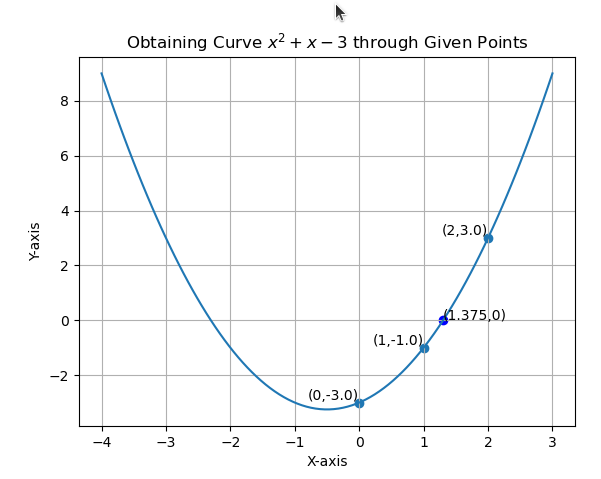
\includegraphics[width=0.7\columnwidth]{figs/fig234.png}
\caption{Parabola passing through given points}
\label{fig:placeholder}
\end{figure}
\end{frame}

\section{Python Code}
\begin{frame}[fragile]
\frametitle{Python Code for Plotting}
\begin{lstlisting}[language=Python]
import numpy as np
import matplotlib.pyplot as plt

# Given points
x_points = np.array([0, 1, 2])
y_points = np.array([-3, -1, 3])

# Find polynomial coefficients (degree 2)
coeffs = np.polyfit(x_points, y_points, 2)

# Create polynomial function
poly = np.poly1d(coeffs)

# Generate x values for smooth curve
x_vals = np.linspace(-4, 3, 100)
y_vals = poly(x_vals)

# Plot curve
plt.plot(x_vals, y_vals)

\end{lstlisting}
\end{frame}
\begin{frame}[fragile]
\begin{lstlisting}
# Plot given points
plt.scatter(x_points, y_points)

label_x = [0, 1, 2]  # points where you want labels
label_y = poly(label_x)

for x, y in zip(label_x, label_y):
    plt.text(x, y, f'({x},{round(y,2)})', fontsize=10,
             ha='right', va='bottom')
   # Add blue dot (same as other points)
plt.scatter(1.3, 0, color='blue')

plt.text(1.3, 0, '(1.375,0)', fontsize=10)

# Labels
plt.xlabel('X-axis')
plt.ylabel('Y-axis')
plt.title('Obtaining Curve $x^2+x-3$ through Given Points')

plt.grid()
plt.show()
\end{lstlisting}
\end{frame}
\begin{frame}[fragile]
\frametitle{Python Code for verification}
\begin{lstlisting}[language=Python]
import numpy as np

# Given points
x_points = np.array([0, 1, 2])
y_points = np.array([-3, -1, 3])

# Find polynomial (degree 2)
coeffs = np.polyfit(x_points, y_points, 2)
poly = np.poly1d(coeffs)

# Print polynomial
print("Polynomial:")
print(poly)

# Verify each point
print("\nVerification:")
for x, y in zip(x_points, y_points):
    y_calc = poly(x)
    print(f"x = {x} -> Calculated y = {y_calc}, Actual y = {y}")

\end{lstlisting}
\end{frame}
\begin{frame}[fragile]
\begin{lstlisting}
# Find values of x when y = 0
roots = np.roots(coeffs)

print("\nValues of x when y = 0:")
for r in roots:
    print(r)

\end{lstlisting}
\end{frame}
\end{document}

